\documentclass[12pt]{beamer}
\usepackage[utf8]{inputenc}
\usepackage[T1]{fontenc}
\usepackage{lmodern}
\usepackage[spanish]{babel}
\usepackage{amsmath}
\usepackage{amsfonts}
\usepackage{amssymb}
\usepackage{graphicx}
% Insertar un gráfico standalone
\usepackage[mode=buildnew]{standalone}
\usetheme{Madrid}
\begin{document}
	\author[Daniel Parra]{Daniel S. Parra G.}
	\title{Simulación PKPD-VK}
	\subtitle{Ivermectina en el tratamiento de infección por SARS-CoV-2}
	%\logo{}
	\institute[UNAL]{Universidad Nacional de Colombia}
	\date{\today}
	%\subject{}
	%\setbeamercovered{transparent}
	%\setbeamertemplate{navigation symbols}{}
	\begin{frame}[plain]
		\maketitle
	\end{frame}
	
	\begin{frame}{Contenido}
		\tableofcontents[currentsection]
	\end{frame}
	
	\section{Introducción}
	\begin{frame}
		\frametitle{Modelo combinado}
		\centering
		\includestandalone[width=1\textwidth]{imagen_tikz}
		
		\bigskip
		\parbox[b]{1.0\textwidth}{\tiny \textbf{Modelo PK}: Duthaler U, Suenderhauf C, Karlsson MO, et al. Population pharmacokinetics of oral ivermectin in venous plasma and dried blood spots in healthy volunteers. Br J Clin Pharmacol 2019; 85: 626–633. \\
			\textbf{Modelo PD}: Caly L, Druce JD, Catton MG, et al. The FDA-approved Drug Ivermectin inhibits the replication of SARS-CoV-2 in vitro. Antiviral Res 2020; 104787.\\
			\textbf{Modelo VK}: Kim KS, Ejima K, Ito Y, et al. Modelling SARS-CoV-2 Dynamics: Implications for Therapy. medRxiv 2020; 2020.03.23.20040493.}
	\end{frame}
	
	\begin{frame}
		\frametitle[PK]{Simulación PK de ivermectina}
		\begin{figure}[t]
			\centering
			%\caption{}
			\label{fig:pk2opcional8}
			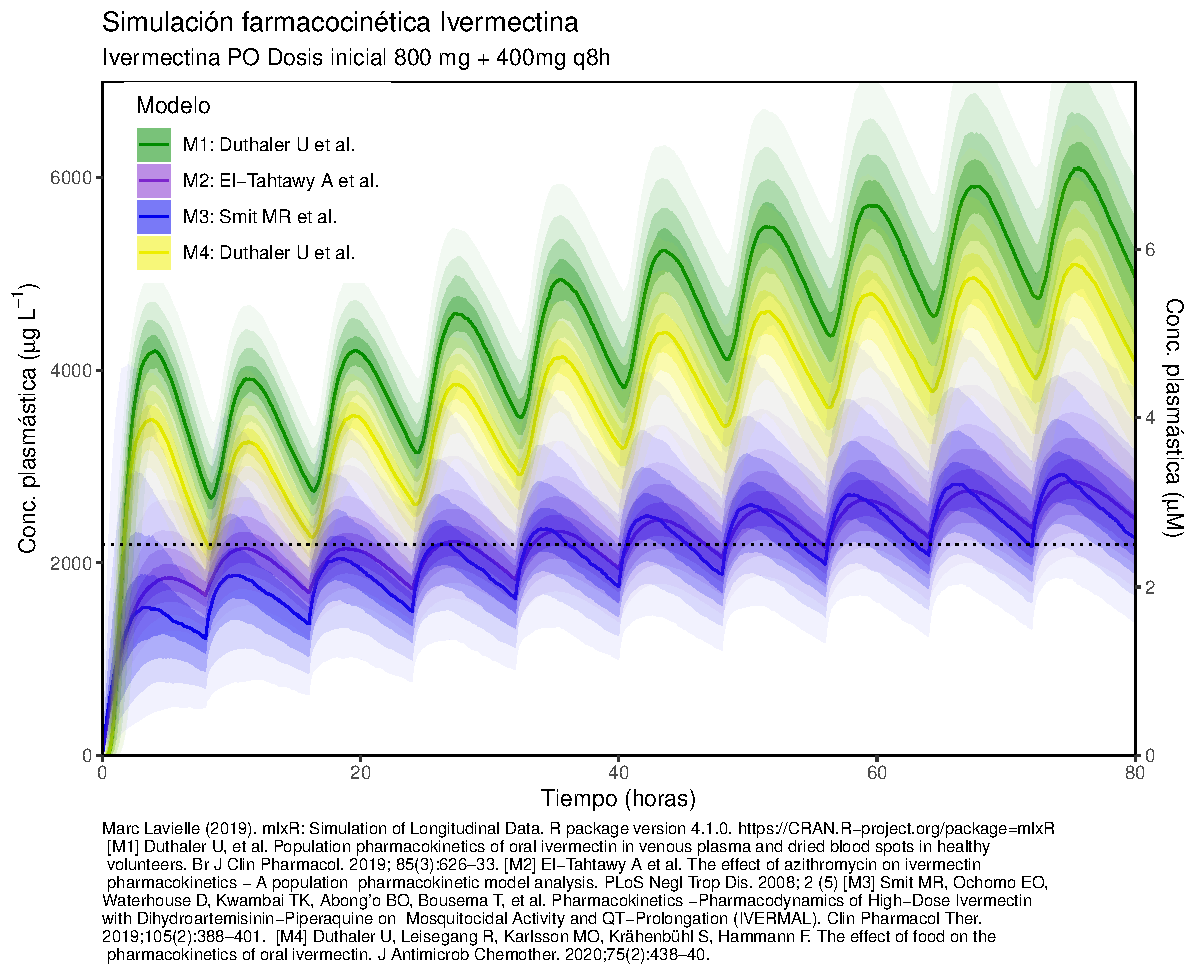
\includegraphics[width=0.8\linewidth]{../modelo_pkpd/PK2_opcional8}
		\end{figure}
	\end{frame}

	\begin{frame}	
		\frametitle{Farmacocinética}			
		\begin{figure}
			\centering
			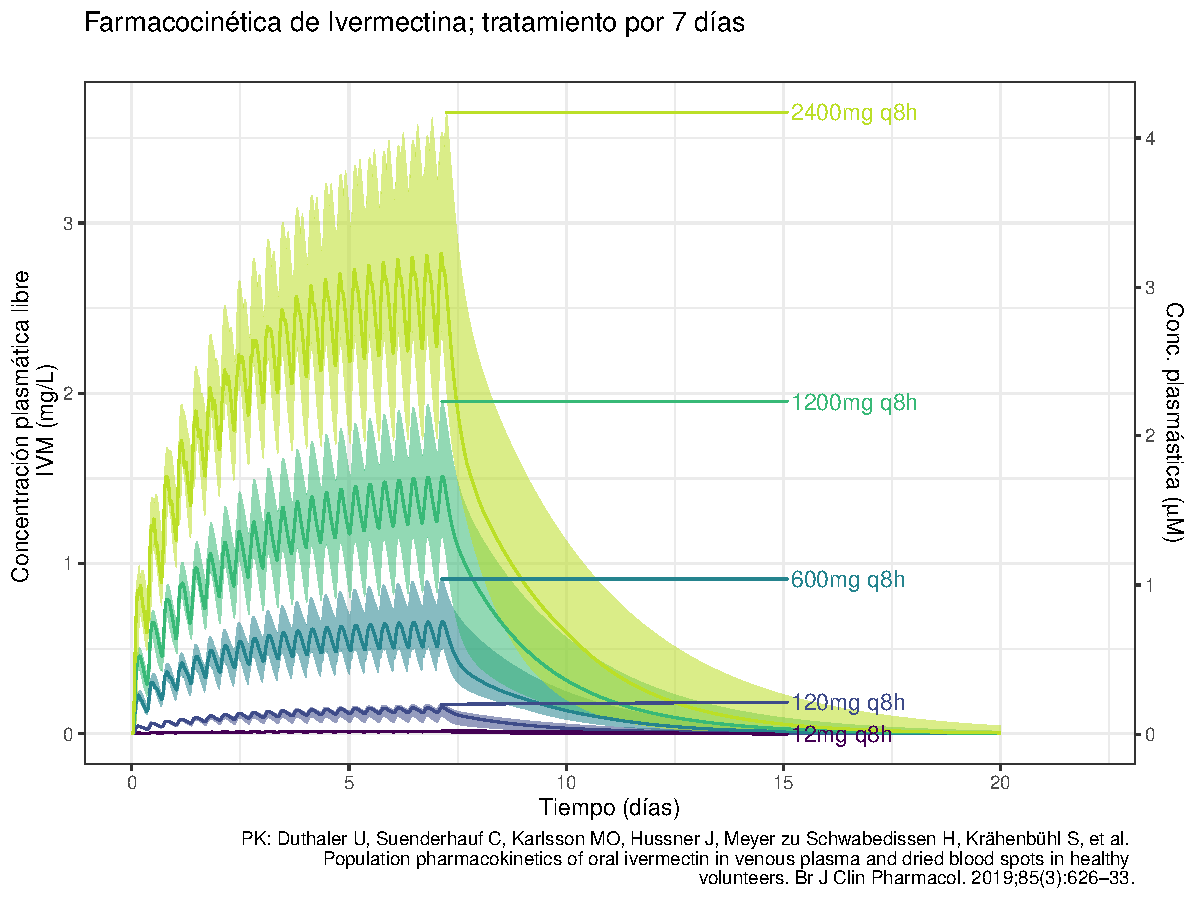
\includegraphics[width=0.9\linewidth]{../modelo_PD_2/figuras/G1}
			%\caption{}
			\label{fig:g1}
		\end{figure}
	\end{frame}
	
	\begin{frame}
		\frametitle{Modelamiento PD ivermectina}
		\begin{figure}
			\centering
			\includegraphics[width=0.8\linewidth]{../modelo_PD/modelo_ivermectina}
			%\caption{}
			\label{fig:modeloivermectina}
		\end{figure}
	\end{frame}
	
	\begin{frame}	
		\frametitle{Farmacodinámica}		
		\begin{figure}
			\centering
			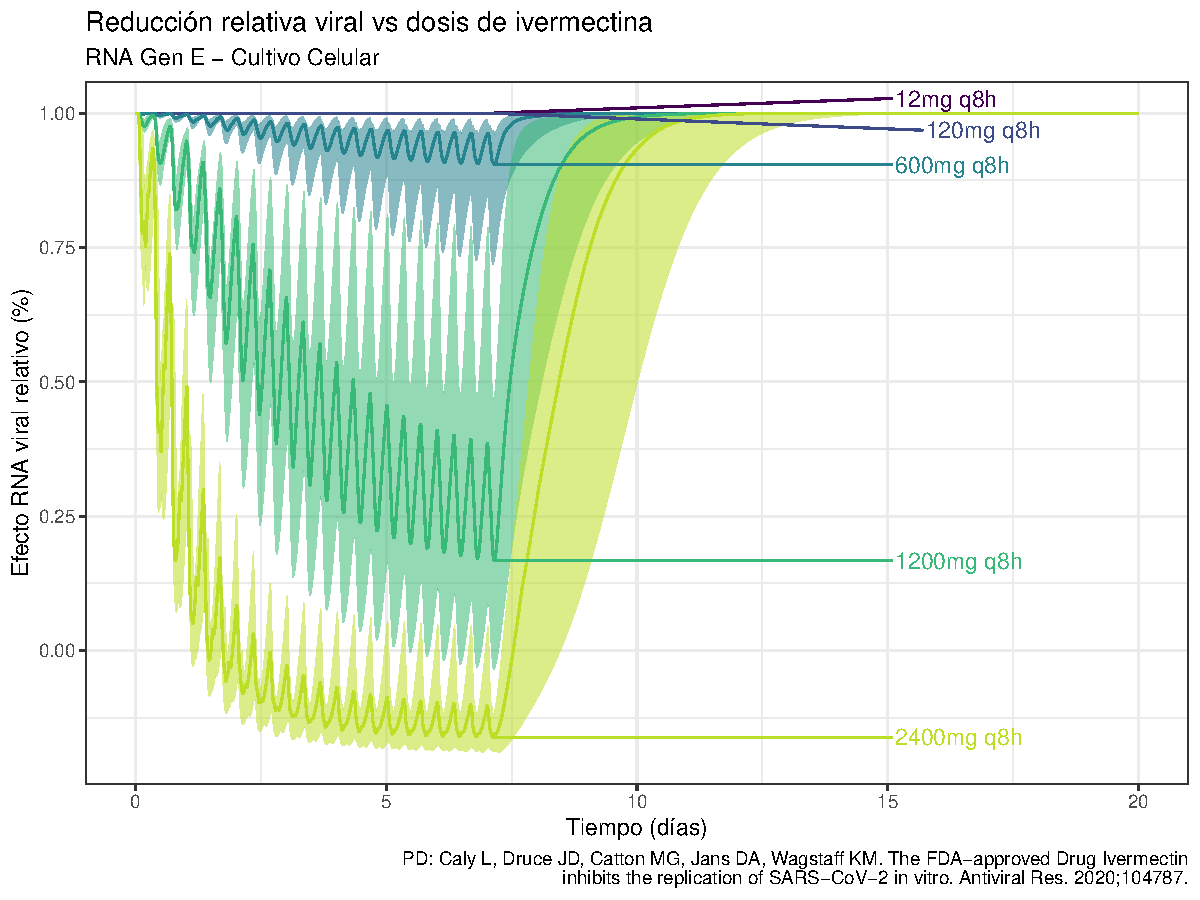
\includegraphics[width=0.9\linewidth]{../modelo_PD_2/figuras/G2}
			%\caption{}
			\label{fig:g1}
		\end{figure}
	\end{frame}
	
	\section{Cinética viral}
	\begin{frame}	
		\frametitle{Cinética viral (1)}		
		\begin{figure}
			\centering
			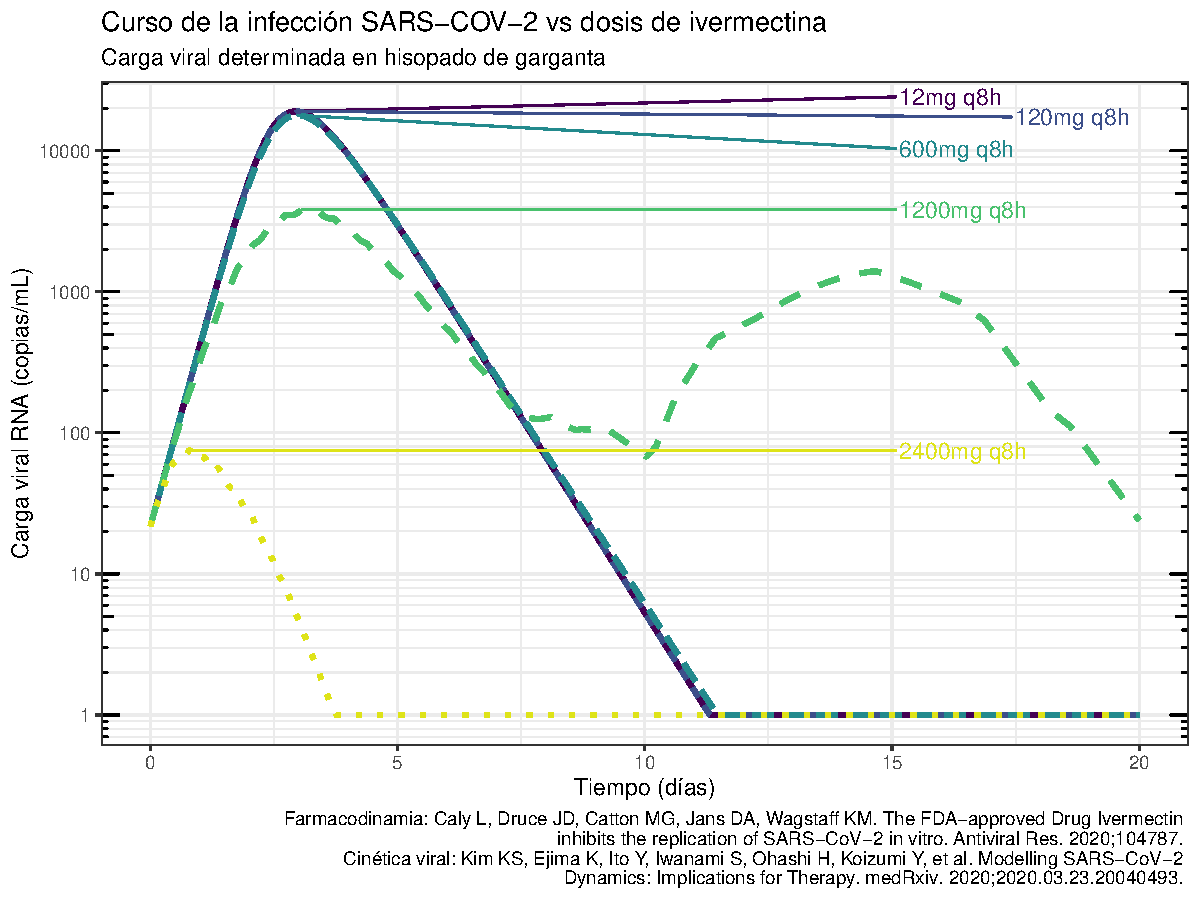
\includegraphics[width=0.9\linewidth]{../modelo_PD_2/figuras/G3}
			%\caption{}
			\label{fig:g1}
		\end{figure}
	\end{frame}

	\begin{frame}	
		\frametitle{Cinética viral (2)}	
		\begin{figure}
			\centering
			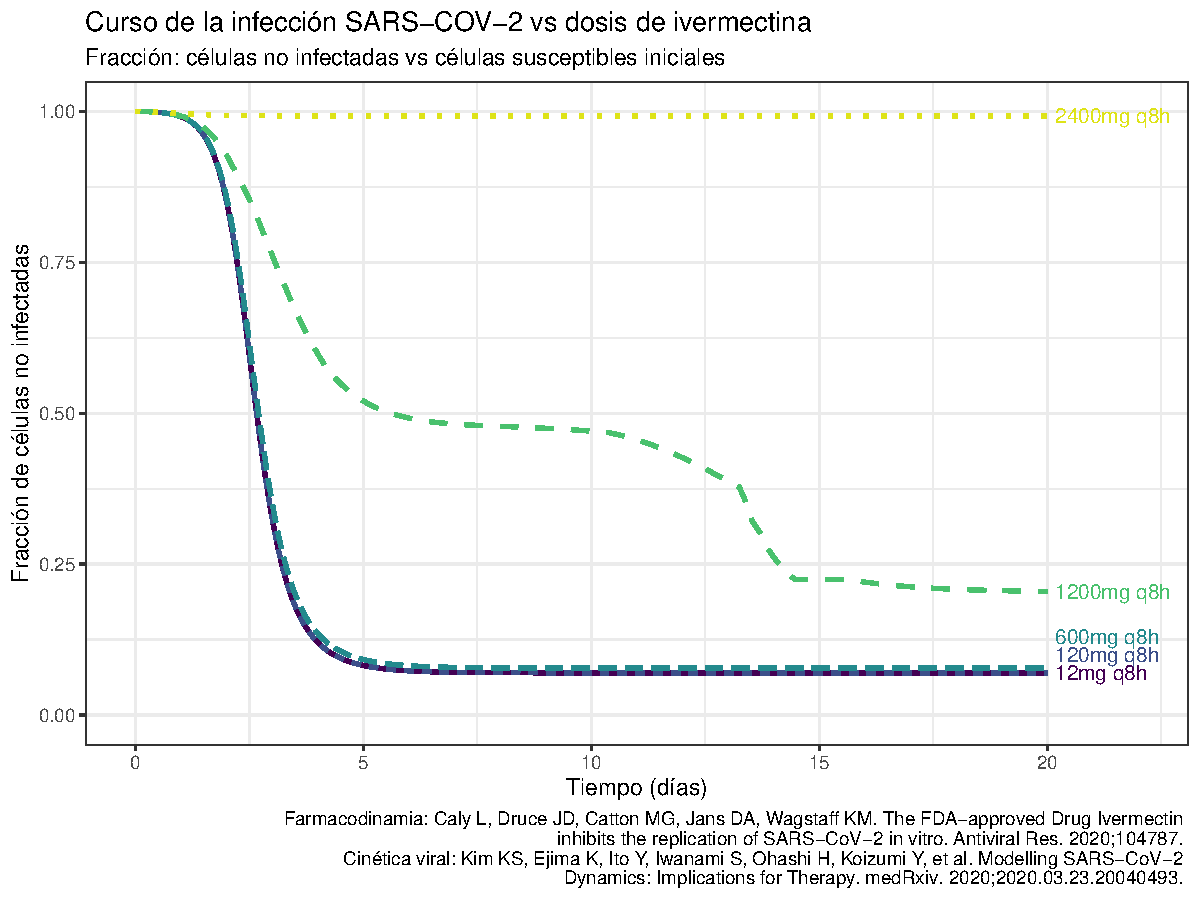
\includegraphics[width=0.9\linewidth]{../modelo_PD_2/figuras/G4}
			%\caption{}
			\label{fig:g1}
		\end{figure}
	\end{frame}
	
	\begin{frame}
		\frametitle[Mapa IVM]{Treemap Ivermectina}
		\begin{figure}[t]
			\centering
			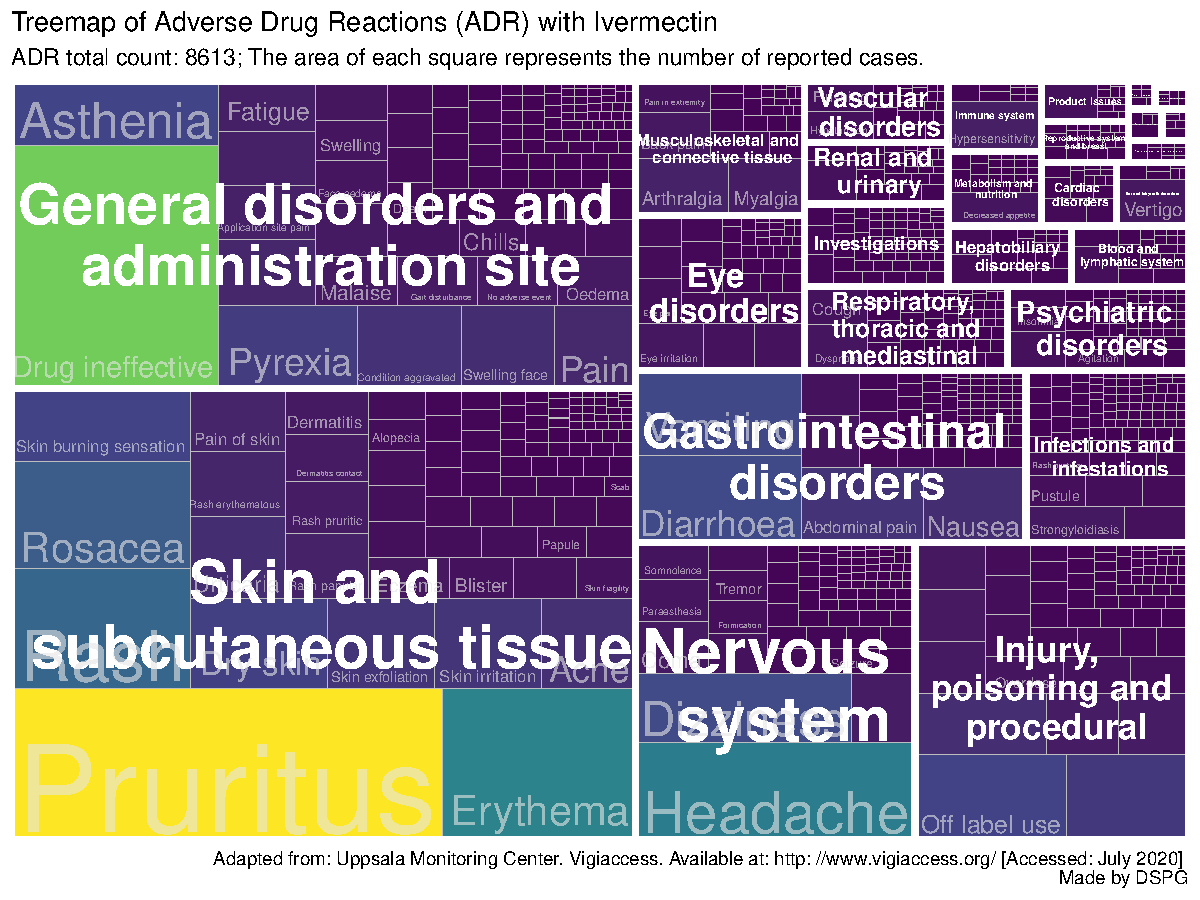
\includegraphics[width=0.8\linewidth]{../seguridad_IVM/Heat_Map_IVM}
%			\caption{\tiny Mapa de árbol de Reacciones Adversas de Medicamentos (RAM) de ivermectina.}
			\label{fig:heatmapivm}
		\end{figure}
	\end{frame}

\end{document}